\section{Data Sources for IPv6 Deployment Measurements}

\subsection{Prefix Allocation Data}

%TODO: introduce notion of prefix!!!
IPv6 Addresses across the internet are allocated by a hierarchy of organisations.
The Internet Assigned Numbers Authority (IANA) have authoritative control of the
allocation of IPv6 addresses, and delegate the allocation of blocks of IPv6
addresses to the five Regional Internet Registries (RIRs), who administer the
address space in their region. The RIR for Europe is Réseaux IP Européens
Network Coordination Centre (RIPE NCC), who in turn are responsible for
allocating addresses to the Local Internet Registries (LIRs).

RIPE NCC keep records of and maintain statistics about all of the IPv6 addresses
allocated since 1999, which can be used to as a metric for how IPv6 is being
deployed, either by counting the number of addresses allocated or by counting
the number of prefixes allocated (recording the number of requests made rather
than the size of subnets asked for). The other RIRs also maintain publicly
available records of their IPv6 and IPv4 prefix allocations, used by Geoff
Huston to generate and maintain historical
reports of IPv6 allocation worldwide, dated from mid-2006 to
present day.

Analysis of this data has been performed by a number of sources. Kuhne tracks
the number of IPv6 allocations from between 1999 and 2010, and identifies three
phases in the allocations of, and hence requests made for IPv6 prefixes since
RIPE started allocating IPv6 addresses. The first phase identified from 1999 to
2002 as "experimental" where IPv6 and the mechanisms to support it were still
under development. The second phase identified between 2002 and 2007 showed
steady but low rates of adoption, that Kuhne contributes to early adopters. The
third phase identified from 2007 to the publication of the data in 2010 showed
an accelerating allocation rate, contributed to the increasing efforts of RIRs
to promote IPv6 in light of the approach of the exhaustion of the IPv4 address
space. The three phases can be seen on the up to date graph of IPv6 allocations
by month from RIPE shown in \ref{fig:alloc-month}. Karpilovsky et al. make
similar conclusion on the allocation data, despite not making recognition of the
experimental phase, Karpilovsky notes that number of allocations was linear
until 2008 when the rate of allocation significantly increased. Karpilovsky et
al. also attempt some analysis of the number of IPv6 address allocated over
time, but find that it is not possible to draw meaningful conclusions from this
data as it is dominated by a very small number of very large allocations.

\begin{figure}[htb]
\centering
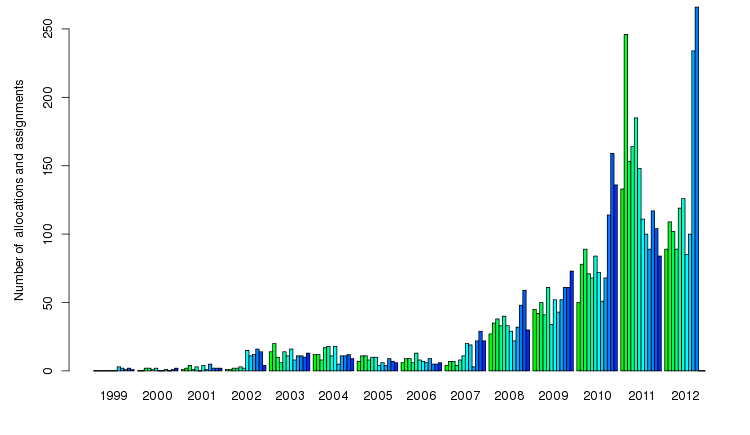
\includegraphics[width=0.4\textwidth]{img/v6-alloc-month.png}
\caption{IPv6 Prefix Allocations by RIPE per month}
\label{fig:alloc-month}
\end{figure}

A factor to consider when thinking about prefix allocation is the difference
between Provider Aggregated (PA) and Provider Independent (PI) addresses. In
IPv6 most unicast addresses are globally aggregatable, to simplify the BGP
routing tables and ensure that the protocol can remain scalable despite the
vastly increased address space. PI addresses remain popular among some
organisations, as they require addresses to remain contiguous across
geographically distant sites, or are not willing to renumber if they change
internet providers. Kuhne notes that following the relaxation of requirements
regarding PI allocation in Feburary 2012, there was a dramatic increase in the 
number of PI allocations.

The use of RIR allocation data as a metric for the deployment of IPv6 at first
seems to be fairly robust, but there are some caveats that must be considered.
Firstly, allocation does not equate to use, and we must turn to other sources of
data to qualify whether the addresses allocated are actually being used. Another
possible issue is that the allocation data published by the RIRs is generally
for allocation to LIRs, so allocation of prefixes to end users is not shown.

%TODO: - haven't looked at Geoff Huston's reports here.

\subsection{BGP Route Data}

Routing of traffic between the individual networks (known as Autonomous
Systems (ASs)) that make up the Internet is performed using the Border Gateway
Protocol(BGP). Each BGP router on the Internet holds routing tables that
detail the ``optimal'' path to all of these networks individual networks.
Each AS announces its existence at the edge of its network, and this
information is propagated across the Internet.

The information held in the routing tables can be used to gain some measure of
the deployment of IPv6, as the routing tables provide an effective summary of
all reachable IPv6 prefixes. This data should give a better view of how IPv6 is
actually being deployed, rather than just the prefixes allocated(CITE).
However, not all prefixes refer to a single AS,
due to route aggregation, a feature of IPv6 designed to reduce the size of the
global routing table by advertising the largest possible prefix where a router
has routes to a number of component prefixes.

- Analysis: papers, delay between allocation and advertisement
- Data Sources: RIPE, potaroo, (CAIDA?)
- v4 comparison
- mention route aggregation at end as an issue?

\subsection{Usage Data}

\subsection{Active Measurements}

\begin{itemize}
    \item Prefix Allocation
    \begin{itemize}
        \item same specifics as BGP Routes
        \item PI vs. PA space, can we measure this?
        \item can relate allocation to use?
    \end{itemize}
    \item BGP Route Data
    \begin{itemize}
        \item sources
        \item analysis of data
        \begin{itemize}
            \item What has been done?
            \item How can we do this?
        \end{itemize}
        \item difficulties and potential problems with the date
    \end{itemize}
    \item Usage Data
    \begin{itemize}
        \item same specifics as BGP Routes
        \item can we measure the extent of tunnelling?
        \item happy eyeballs
        \item browser configuration (re: dual stack)
    \end{itemize}
    \item Active Measurements
    \begin{itemize}
        \item same specifics as BGP Routes
        \item Atlas and Ark
        \item how does this add to the existing other data sets?
    \end{itemize}
\end{itemize}
